\section{Filtro 2: Merge}

\subsection{Cambios}
Para el recuperatorio decidimos hacer cambios en el codigo.

La lista de cambios esta a continuacion, con la aclaracacion de por que se hicieron los mismos:
\noindent
\begin{itemize}
\item Se elimino uno de los iteradores de ciclo para reducir la cantidad de saltos condicionales y mejorar la performance del codigo.
\item En la primera implementacion cambio la utilizacion de \texttt{CALL addPixels} por un macro debido a que los calls rompen el pipeline y requieren operaciones extra.
\item Se cambio la escritura a disco de usar \texttt{PEXTRD}, \texttt{PINSRD} y luego hacer MOVDQU de un solos registro \texttt{XMM} a hacer \texttt{MOVD} del registro \texttt{XMM0} luego de cada llamada del macro addPixels
\end{itemize}

En la experimentacion se ve que los cambios no producen una mejora de performance notable pero decidimos dejarlos por que ayudaban a hacer el codigo mas claro para leer y por que a pesar de que fueron optimizaciones fallidas concideramos que los resultados inesperados que devolvio la experimentacion son importantes.

\subsection{Explicacion}
El filtro $merge$ consiste en tomar 2 imagenes del mismo tamaño y un parametro (llamdo \texttt{value} en el enunciado) de tipo $float$ entre 0 y 1, multiplicar las componetes de la primer imagen por \texttt{value} y los de la segunda por \texttt{1 - value} y sumar los pixeles de ambas para crear una nueva imagen. \\

\subsection{Implementacion 1}
Para la primer implementacion se nos pidio trabajar con valores de tipo $float$, procesando la mayor cantidad de pixeles posibles por iteracion. \\

Ya que la cantidad de pixeles por imagen siempre va a ser un multiplo de 4 segun el enunciado, decidimos tomar de a 4 pixeles de la memoria para trabajar con los mismos, esto nos permitio simplificar el ciclo y operar sin tener que preocuparnos por excedernos del area de memoria alocada a la imagen.\\

Para procesar los pixeles del merge utilizamos 2 registros \texttt{XMM} para guardar los 4 pixeles como bytes que obtenemos de la memoria, y 2 registros mas para guardar copias de los mismos. Ademas como utilizamos un macro tambien precisamos de 4 registros \texttt{XMM} mas para poder guardar los resultados de la funcion. Por ultimo, tenemos \texttt{value} y \texttt{1 - value} guardados en los registros \texttt{XMM15} y \texttt{XMM14} respectivamente. Ademas de estos registros, se emplearon tambien los siguientes de proposito general:\\

\noindent
\begin{itemize}
	\item \texttt{RDX} puntero a la primera imagen
	\item \texttt{RCD} puntero a la segunda imagen
	\item \texttt{R9} cantidad de bytes totales de la imagen
	\item \texttt{R8} contador
\end{itemize}

Esta distribucion de registros reponde al siguiente grafico:

\begin{figure}[h!]
	\centering
	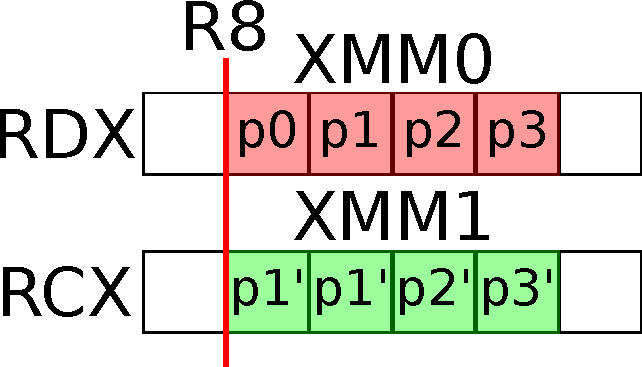
\includegraphics[scale=0.5]{images/MergeASM1_0}
\end{figure}

Antes de empezar a recorrer la imagen, para asignar los valores correctos de \texttt{XMM14} y \texttt{XMM15} utilizamos el dato \texttt{value} original almacenado en \texttt{XMM0}. Esto lo hacemos mediante una operacion de shuffle hacia \texttt{XMM15}, la misma copia \texttt{value} a todas las componentes de \texttt{XMM15}. Para poder calcular \texttt{XMM14} alcanzo con mover al mismo una constante almacenada en memoria que tuviese \texttt{1.0} en los 4 $float$ y posteriormente restarle el contenido de \texttt{XMM15}. Finalmente tenemos en \texttt{XMM14} y \texttt{XMM15}:\\

\noindent
\texttt{XMM14 $\gets$ 1 - value $\vert$ 1 - value $\vert$ 1 - value $\vert$ 1 - value}\\
\texttt{XMM15 $\gets\ \ $ value $\ \ \vert\ \ $ value $\ \ \vert\ \ $ value $\ \ \vert\ \ $ value}\\

Para poder movernos por la imagen empleamos un ciclo, iteramos sobre el la imagen de a 16 bytes usando \texttt{R8} como contador. Antes de comenzar a iterar incializamos \texttt{R8} en 0. Al comienzo de cada ciclo, movemos hacia los registros \texttt{XMM0} y \texttt{XMM1} los datos de los pixeles a procesar de la primer y segunda imagen respectivamente, ademas copiamos cada una en \texttt{XMM2} y \texttt{XMM3}, luego de esto procedimos a llamar al macro \texttt{addPixels} 4 veces. Al finalizar los llamados, tenemos en \texttt{XMM4} los 4 pixeles procesados, lo unico restante fue volcarlos en memoria. Una vez que los pixeles se encuentran en memoria, tenemos que aumentar el contador 16 bytes, tambien aumentamos los punteros a la imagenes por el mismo valor y luego comparo \texttt{R8} con \texttt{R9}. Si ya llegue al final de la imagen, termino el ciclo de la implementacion y procedo a retornar de la funcion.

El macro \texttt{addPixels} es una funcion auxiliar la cual hace la aritmetica necesaria para poder mergear las imagenes, esta funcion toma los valores de \texttt{XMM2} y \texttt{XMM3} y los copia hacia \texttt{XMM0} y \texttt{XMM1} respectivamente, luego procede a desempaquetarlos a doubleword utilizando el registro \texttt{XMM10} el cual contiene 0 en todas sus componentes. Una vez desempaquetados los valores, se procede a convertirlos a tipo $float$ para poder realizar el producto con \texttt{XMM14} (\texttt{1-value}) y \texttt{XMM15} (\texttt{value}). Entonces tenemos:

\noindent
\texttt{XMM0 $\gets$ a * value $\vert$ r * value $\vert$ g * value $\vert$ b * value}
\texttt{XMM1 $\gets$ a * (1 - value) $\vert$ r * (1 - value) $\vert$ g * (1 - value) $\vert$ b * (1 - value)}

Con estos valores en los registros, lo unico restante es sumarlos, convertirlos nuevamente a entero, y empaquetarlos a byte. Antes de finalizar la funcion, shifteamos los registros \texttt{XMM2} y \texttt{XMM3} 4 bytes a la derecha, asi en el siguiente llamado al macro ya van a estar los siguientes pixeles a procesar en el lugar correcto.

\subsection{Implementacion 2}
Para la segunda implementacion se no pidio trabajar con enteros procesando la mayor cantidad de enteros posibles por iteracion. Al igual que en la primera implementacion trabajamos de a 4 pixeles al mismo tiempo por que nos permite iterar de manera segura. Al igual que antes vamos a emplear los registros \texttt{XMM14} y \texttt{XMM15} para guardar los valores por los cuales vamos a multiplicar los pixeles. Para calcularlos movimos \texttt{value} a XMM15, luego aplicamos un shuffle para que los 4 floats de \texttt{XMM15} \texttt{value}, luego movimos a \texttt{XMM14} una constante de $float$ almacenada en memoria la cual contenia \texttt{8192.0} en cada una de sus componentes, este registro fue multiplicado por \texttt{XMM15} almacenando el resultado del producto en \texttt{XMM15}, para obtener el \texttt{1 - value} lo unico necesario fue restarle a \texttt{XMM14} el contenido de \texttt{XMM15}. Finalmente tenemos:\\

\noindent
\texttt{XMM15 $\gets$ 8192.0 * value $\vert$ 8192.0 * value $\vert$ 8192.0 * value $\vert$ 8192.0 * value}\\
\texttt{XMM14 $\gets$ 8192.0 - 8192.0 * value $\vert$ 8192.0 - 8192.0 * value $\vert$ 8192.0 - 8192.0 * value $\vert$ 8192.0 - 8192.0 * value}\\
\texttt{XMM14 $\gets$ 8192.0 *(1 - value) $\vert$ 8192.0 * (1 - value) $\vert$ 8192.0 * (1 - value) $\vert$ 8192.0 * (1 - value)}\\

El numero 8192, que es $2^{13}$ fue elegido de manera empirica, ya que era el numero mas pequeño que nos permitia que el margen de error fuese lo suficientemente pequeño para poder cumplir con el enunciado.

Ademas de estos registros vamos a emplear los mismos registros de proposito general que la primer implementacion, junto con los registros \texttt{XMM0} a \texttt{XMM7} para tomar los valores de la imagen de la memoria y desempaquetar.

\begin{figure}[h!]
	\centering
	\includegraphics[scale=0.5]{images/MergeASM2_0}
\end{figure}

La estructura de la primera implementacion se mantuvo igual, es decir, se preservo el ciclo y el uso del contador, esto significa que las misma precauciones respecto a los mismos tomadas anteriormente aplican nuevamente en ese caso. Una vez dentro del ciclo procedimos a mover hacia \texttt{XMM0} y \texttt{XMM4} los grupos de pixeles de la primera y segunda imagen respectivamente. Estos fueron desempaquetados a doubleword, quedando de la siguiente forma:

\noindent
\texttt{XMM0 $\gets$ p0}\\
\texttt{XMM1 $\gets$ p1}\\
\texttt{XMM2 $\gets$ p2}\\
\texttt{XMM3 $\gets$ p3}\\
\texttt{XMM4 $\gets$ p0'}\\
\texttt{XMM5 $\gets$ p1'}\\
\texttt{XMM6 $\gets$ p2'}\\
\texttt{XMM7 $\gets$ p3'}\\

Despues se multiplico a \texttt{XMM0}, \texttt{XMM1}, \texttt{XMM2} y \texttt{XMM3} por \texttt{XMM15}, el resultado de la operacion fue shifteado 14 bits hacia la derecha, obteniendo \texttt{(p * 8192 * v) / 8192 = p * v}. Esta misma logica se aplico con los otro cuatro registros, salvo que fueron multiplicados por \texttt{XMM14}, obteniendo \texttt{(p * 8192 * (1 - v) / 8192 = p * (1 - v)}. Una vez completado esto, finalmente tenemos cada pixel multiplicado por su \texttt{value} correspondiente, los mismos luego fueron empaquetados en un solo registro como muestra el grafico:

\begin{figure}[h!]
	\centering
	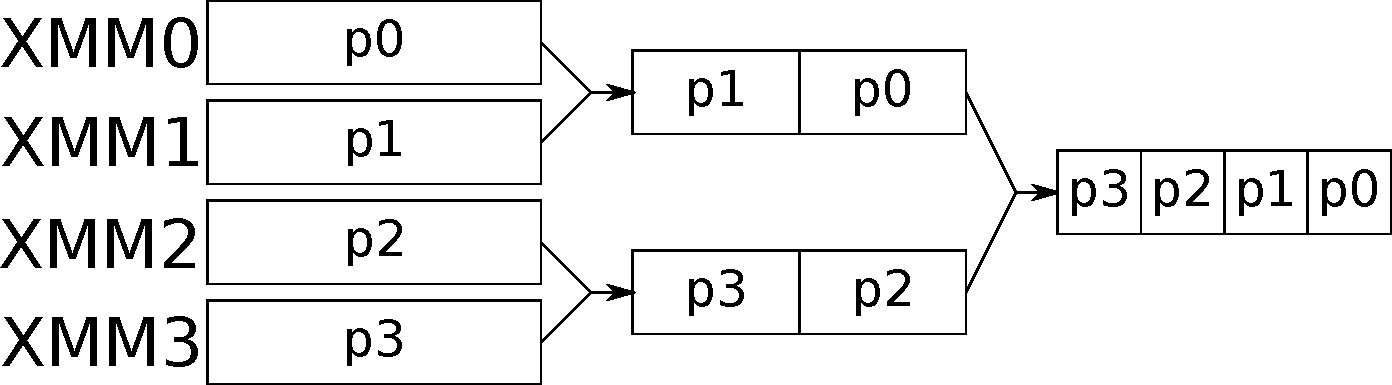
\includegraphics[scale=0.5]{images/MergeASM2_1}
\end{figure}

Al final tenemos:\\

\noindent
\texttt{XMM0 $\gets$ p3 * value $\vert$ p2 * value $\vert$ p1 * value $\vert$ p0 * value}\\
\texttt{XMM4 $\gets$ p3' * (1 - value) $\vert$ p2' * (1 - value) $\vert$ p1' * (1 - value) $\vert$ p0' * (1 - value)}\\

Para terminar solo fue necesario sumarlos y moverlos a memoria.

\newpage
\subsection{Resultados}
Para la experimentacion de $merge$ se empleo la misma metodologia que en el caso de $blur$. El resultado obtenido fue el siguiente:

\begin{figure}[h!]
	\centering
	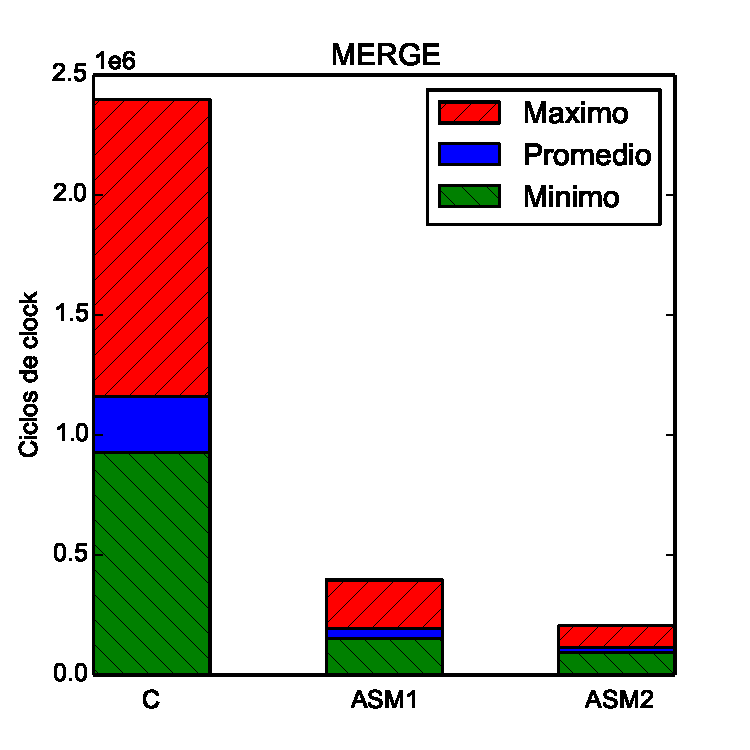
\includegraphics[scale=0.45]{images/merge_comparation}
\end{figure}

Al igual que en el caso de $blur$ el uso del paralelismo de SIMD impacto positivamente en el rendimiento, las dos implementaciones con SSE terminaron siendo mas eficientes que la de $C$. Como era de esperar, en el caso de $ASM1$, el costo de conversion a $float$ termino impactando negativamente el rendimiento en un margen pequeño.

Al igual que con $blur$, decidimos correr las implementaciones de la primer entrega y compararlas con las nuevas. Terminamos obteniendo:

\begin{figure}[h!]
	\centering
	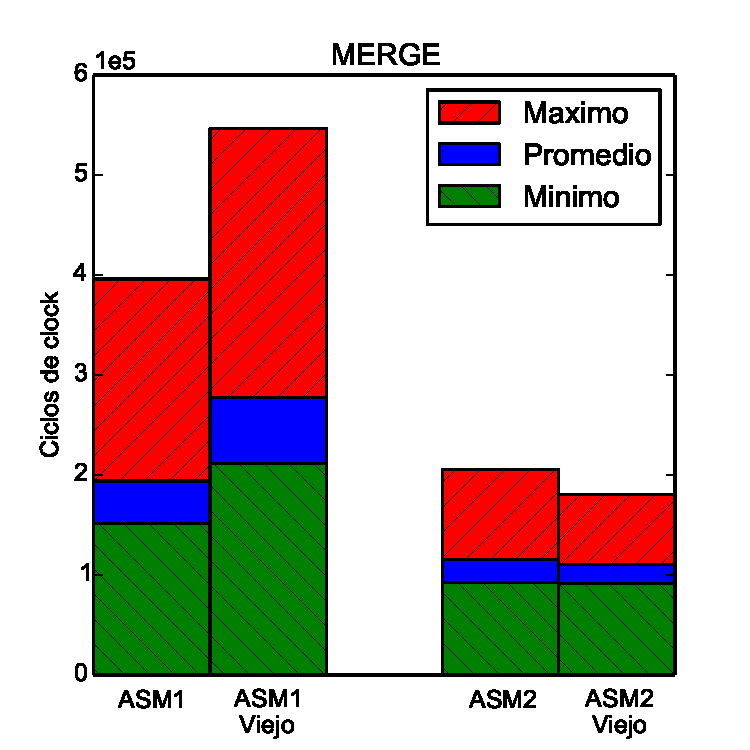
\includegraphics[scale=0.45]{images/merge_comparationOLD}
\end{figure}

Esta experimentacion nos sorprendio ya que la eliminacion de branches tanto con los calls como con los jumps practicamente no cambio el tiempo de ejecucucion del programa, en caso de $ASM1$ el cambio que vemos es principalmente motivado por la manera en la que ahora hacemos el pasaje a memoria.

\newpage
Luego de descubrir que la operacion \texttt{PEXTRD} y \texttt{PINSRD} son operaciones caras (Requieren varios ciclos de clock) decidimos probar si era mas rapido usar estas instrucciones o hacer 4 copias a memoria directamente desde el registro \texttt{XMM} usando \texttt{MOVD}.

\begin{figure}[h!]
	\centering
	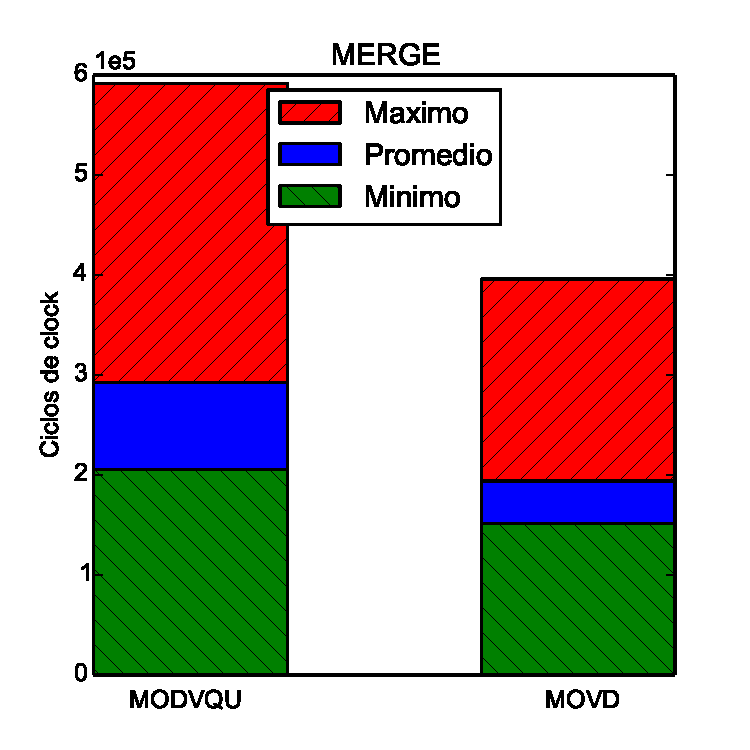
\includegraphics[scale=0.45]{images/merge_extractmov}
\end{figure}

Con esto podemos ver que las operaciones de extraccion e insercion de codigo son mas caras que hacer los 4 accesos a memoria.

% Para la experimentacion vamos a correr las 3 implementaciones (La version de $C$ compilada con optimizaciones de nivel 3) con la imagen de $lena$ brindada por la catedra (multiplos de 16x16, hasta 320x320), se corren 100 veces cada tamaño y despues se saca un promedio y se grafica el maximo, el minimo y el promedio.

% \begin{figure}[h!]
% 	\centering
% 	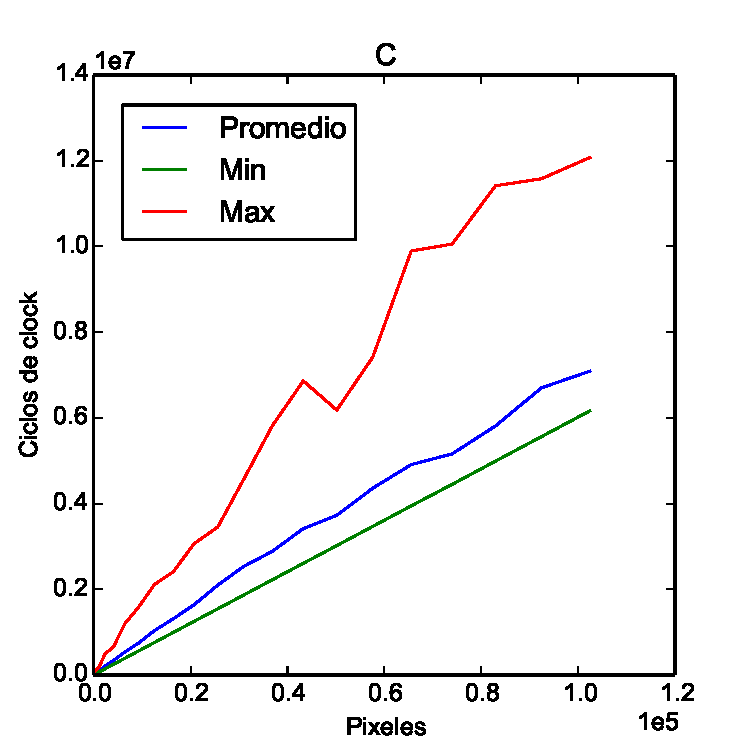
\includegraphics[scale=0.45]{images/c_merge}
% 	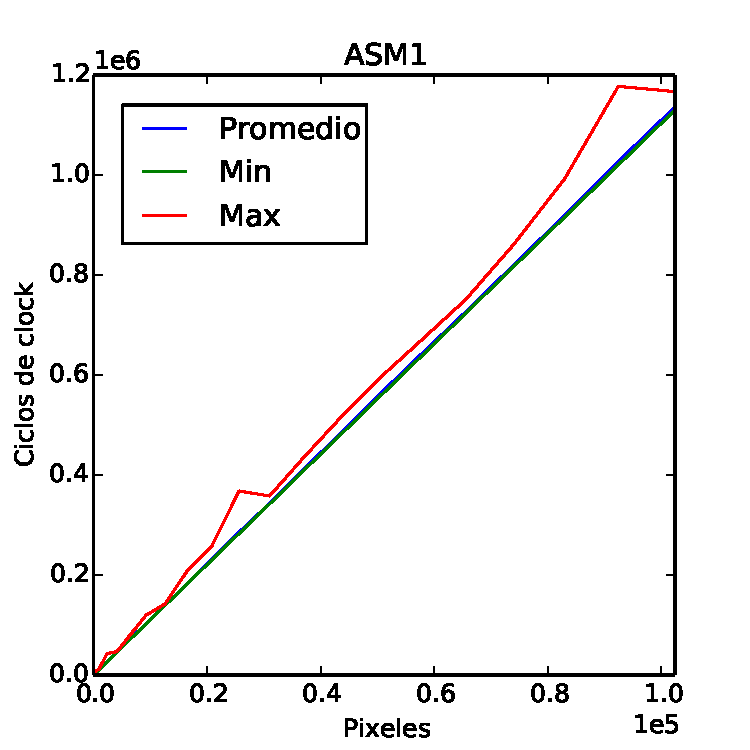
\includegraphics[scale=0.45]{images/asm1_merge}
% 	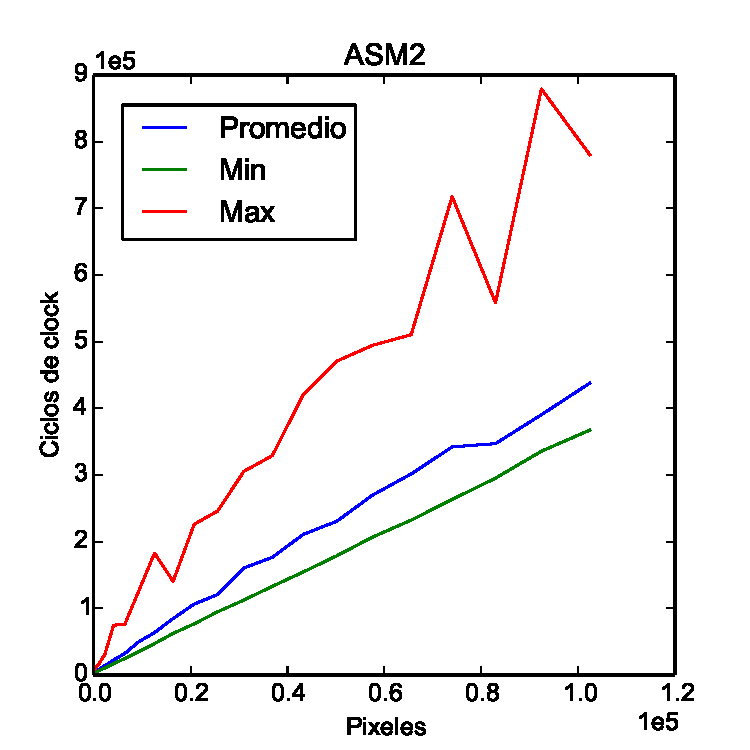
\includegraphics[scale=0.45]{images/asm2_merge}
% \end{figure}

% Tambien graficamos los 3 promedios en un grafico para ver cual de ellos es el mas rapido en general. Y para ver mejor la diferencia entre ASM1 y ASM2 los graficamos aparte.

% \begin{figure}[h!]
% 	\centering
% 	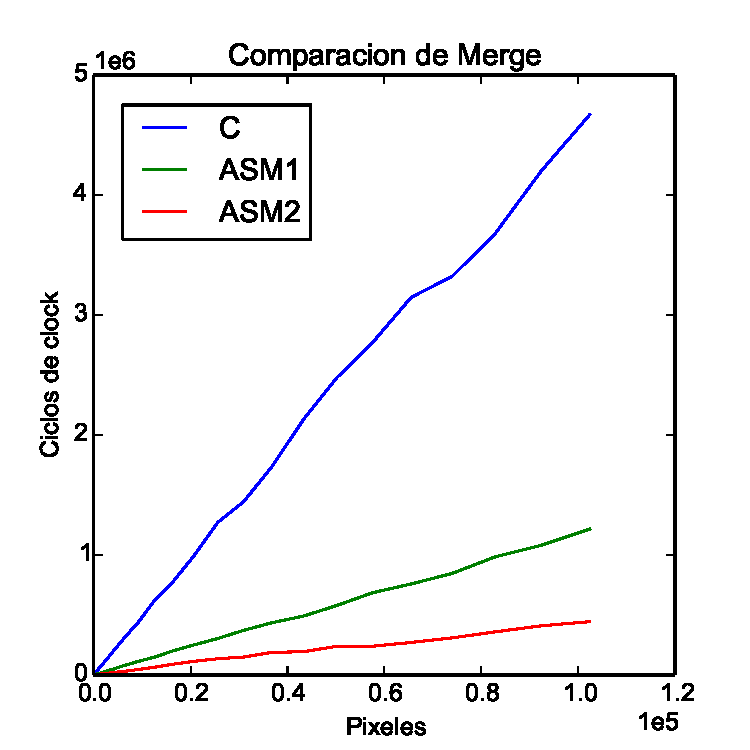
\includegraphics[scale=0.5]{images/c_asm1_asm2_merge_comp}
% 	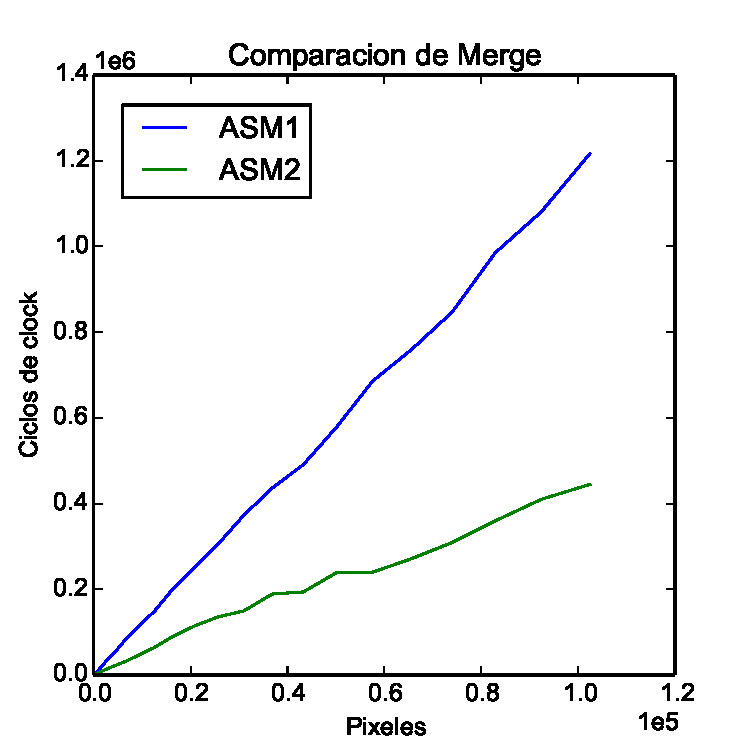
\includegraphics[scale=0.5]{images/asm1_asm2_merge_comp}
% \end{figure}
% \newpage

% Tambien queremos ver que la imagen no modifique el tiempo de ejecucion, tanto el codigo de C como el de ASM no poseen ningun salto condicional que depende de el valor de los pixeles.

% \begin{figure}[h!]
% 	\centering
% 	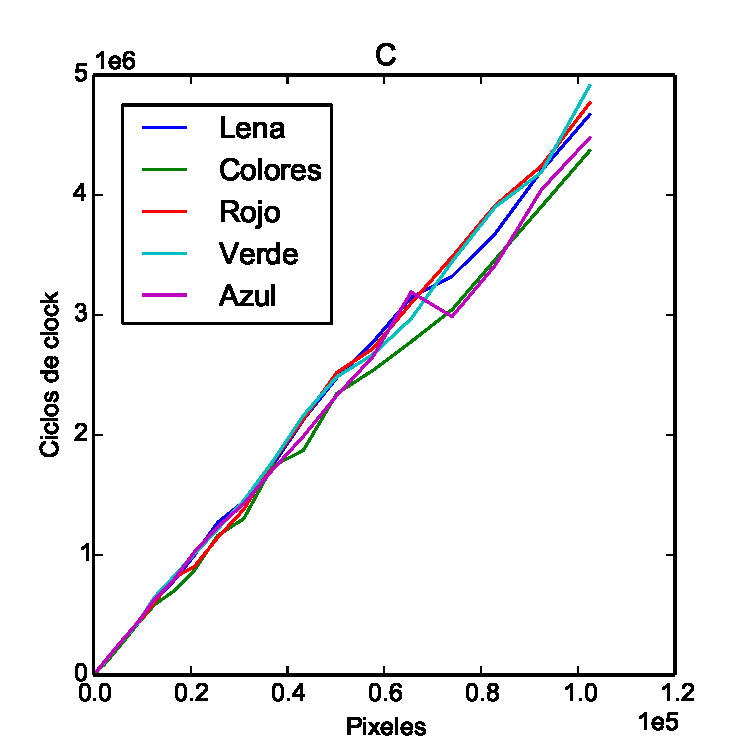
\includegraphics[scale=0.45]{images/c_merge_lena_colors}
% 	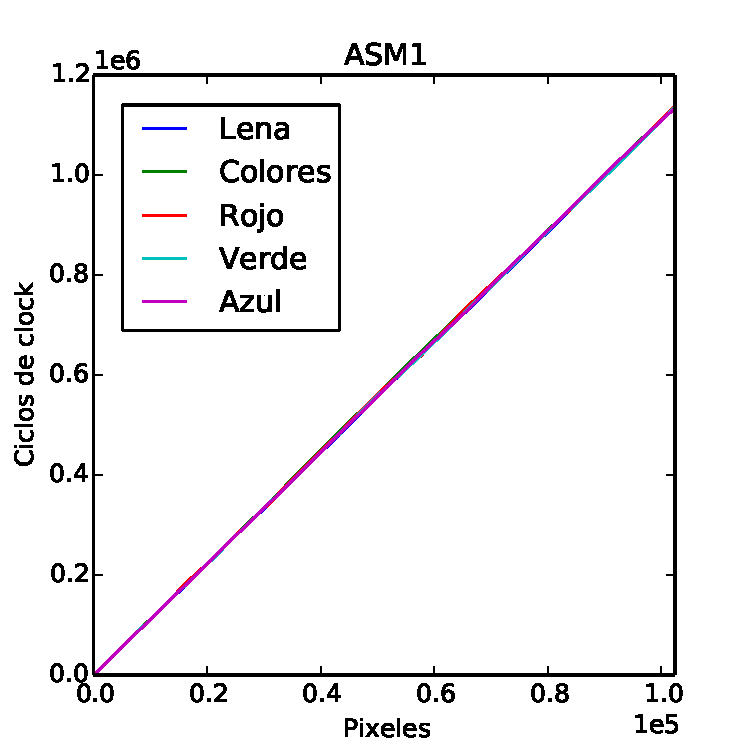
\includegraphics[scale=0.45]{images/asm1_merge_lena_colors}
% 	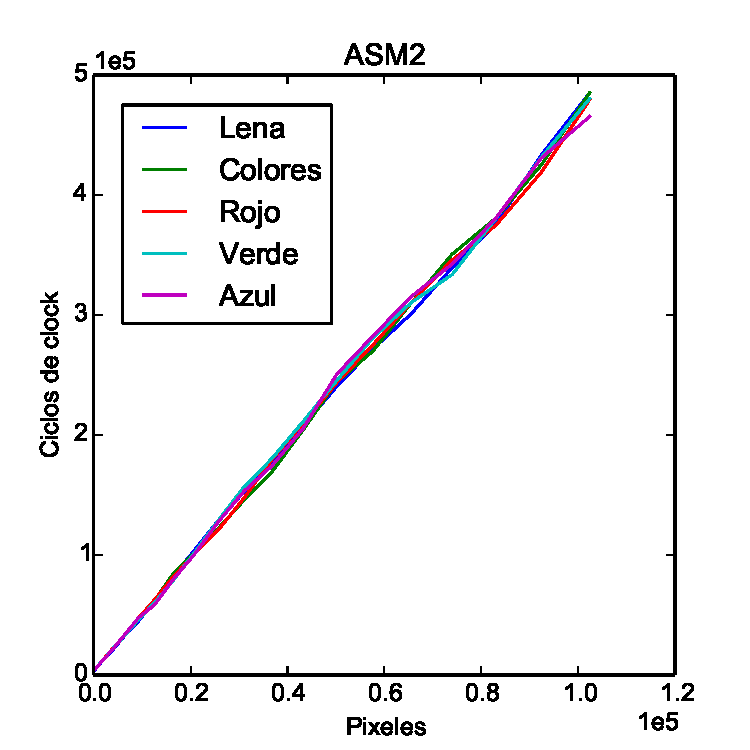
\includegraphics[scale=0.45]{images/asm2_merge_lena_colors}
% \end{figure}

\subsection{Conclusion}

En el caso de $merge$ podemos volver a apreciar la eficiencia de utilizar SIMD en la implementacion, en este caso incluso la diferencia es mas marcada que en el de $blur$, particularmente por la simpleza del algoritmo en si. Tal como esperabamos, la implementacion utilizando $float$ via conversiones termino tomando mas ciclos de reloj que la que se maneja directamente con numeros enteros. Por ultimo, consideramos importante destacar la efectividad del predictor de saltos, ya que este minimizo efectivamente el costo de los mismos.

% Al igual que en el primer filtro, las implementacion de $Assembler$ terminaron siendo mas veloces que la de $C$. La consistencia de los resultados tambien nos lleva a concluir que el costo en tiempo de hacer las conversiones en la primer implementacion es considerable, ya que la segunda version, al estar realizada sobre enteros minimizando las operaciones de punto flotante, tardo considerablemente menos.	